\section{Epilogue}

\begin{frame}{Lessons \& Philosophy: Adaptation in Life}
  \centering
  \vspace{3em}
  \begin{tikzpicture}
    \draw [thick] [<->] (0,6) node [left] {Happiness}
    -- (0,0) --
    (6,0) node [below] {Money};

    \foreach \Point in {(5.5, 5.5), (5, 5.2), (4.5, 4.9), (4, 4.5), (3.8, 4.3)}{
      % \node<+-> [ACMBlue] at \Point {x};
      \node [ACMBlue] at \Point {x};
    }
  \end{tikzpicture}
\end{frame}

\begin{frame}{Acknowledgment}

  \begin{figure}
    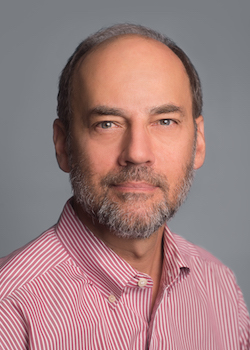
\includegraphics[width=0.15\linewidth]{figures/lee.jpg}
    \pause
    \hfill
    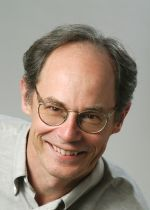
\includegraphics[width=0.15\linewidth]{figures/wawrzynek.jpg}
    \hfill
    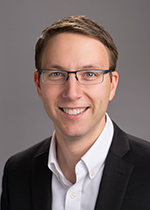
\includegraphics[width=0.15\linewidth]{figures/hartmann.jpg}
    \hfill
    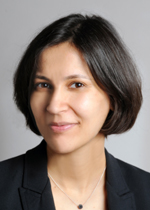
\includegraphics[width=0.15\linewidth]{figures/ratnasamy.jpg}
    \hfill
    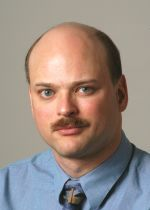
\includegraphics[width=0.15\linewidth]{figures/kubiatowicz.jpg}
    \hfill
  \end{figure}

  \begin{columns}
    \column{0.15\textwidth}
    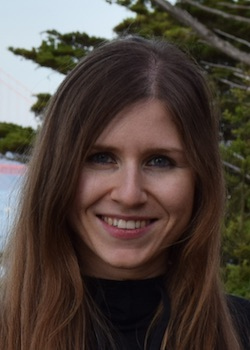
\includegraphics[width=0.9\linewidth]{figures/akkaya.jpg}
    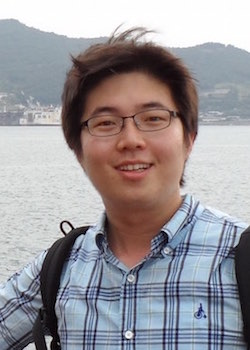
\includegraphics[width=0.9\linewidth]{figures/kim.jpg}

    \column{0.15\textwidth}
    
\includegraphics[width=0.9\linewidth]{figures/shaver.jpg}
    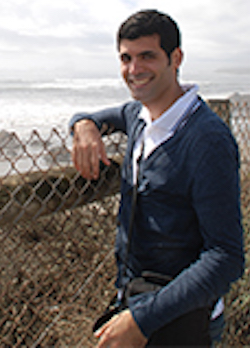
\includegraphics[width=0.9\linewidth]{figures/iannopollo.jpg}

    \column{0.7\textwidth}
    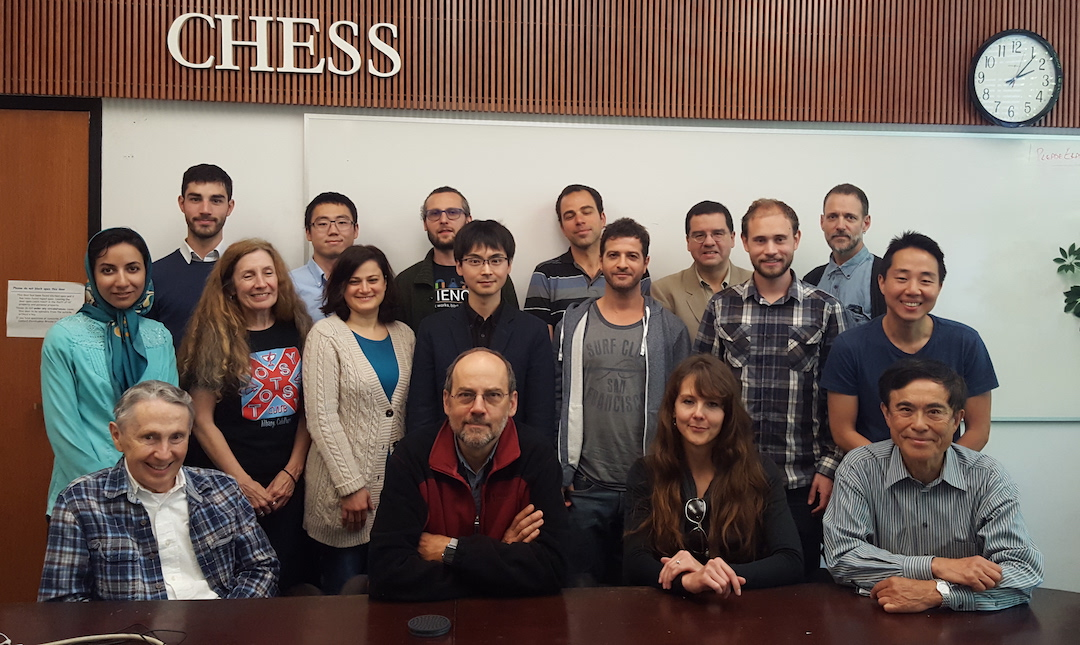
\includegraphics[width=0.9\linewidth]{figures/ptolemy_group.jpg}
  \end{columns}

\end{frame}

%%% Local Variables:
%%% mode: latex
%%% TeX-master: "talk"
%%% TeX-engine: xetex
%%% End:
